\section{Image Transformations for Feature Extraction}

\subsection{The Gabor Filter}

In content based image retrieval, the inability of the Fourier transform to
localize the frequency components in time disqualifies it as a suitable
analysis method. Instead, wavelets are often used to obtain a time-frequency
representation of the signal. A particulaly successful application to CBIR was
the use of gabor wavelets as proposed by Manjunath and Ma
\autocite{manjunath_texture_1996}. The mother Gabor wavelet $g(x, y)$ with the
sinus frequency $W$ and gaussian scaling parameters $\sigma_x$, $\sigma_y$ is
given as
\begin{equation*}
    g(x, y) = \left( \frac{1}{2 \pi \sigma_x \sigma_y} \right) \exp{\left( - \frac{1}{2} \left( \frac{x^2}{\sigma_x^2} + \frac{y^2}{\sigma_y^2} \right) + i \cdot 2 \pi W x \right)}
\end{equation*}
and thus its Fourier transform as
\begin{equation*}
    \hat{g}(u, v) = \exp{\left( - \frac{1}{2} \left( \frac{(u - W)^2}{\sigma_u^2} + \frac{v^2}{\sigma_v^2} \right) \right)}\text{, }
    \sigma_u = \frac{1}{2} \pi \sigma_x \text{ and } \sigma_v = \frac{1}{2} \pi \sigma_y
\end{equation*}
The individual wavelets $g_{m, n}(x, y)$ are generated from $g(x, y)$ by
scaling and rotation by $\theta = \frac{n \pi}{K}$ for all $0 < n < K$
orientations:
\begin{equation*}
    g_{m, n}(x, y) = a^{-m} g \left( a^{-m} (x \cos{\theta} + y \sin{\theta}), a^{-m} (-x \sin{\theta} + y \cos{\theta}) \right).
\end{equation*}
To avoid redundancy due to overlap, the scaling parameters $\sigma_u$ and
$\sigma_v$ are chosen in a way that the frequency spectra can be tiled as in
figure \ref{fig:gabor_tiling}. A normalization to zero mean can be added to
remove the influence of the input's intensity value scale.

The individual coefficients can be obtained by convolving each filter of the
filter bank with the signal.

\begin{figure}[h]
    \centering
        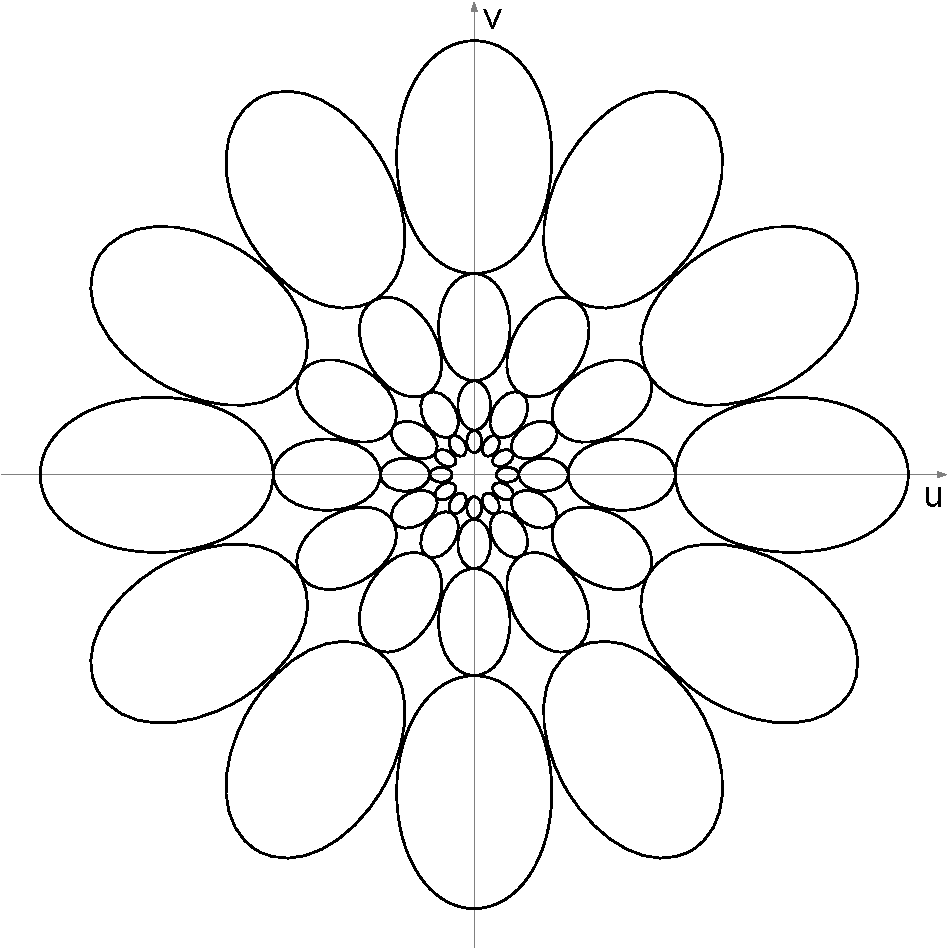
\includegraphics[width=0.5\textwidth]{gabor_tiling_cropped}
    \caption[Tiling of Gabor wavelets]{
        Tiling of Gabor wavelets. Note that due to the elliptical shape of the
        wavelets, some parts of the spectrum are left uncovered. (Image
        inspired by Manjunath and Ma \autocite{manjunath_texture_1996})
        }
    \label{fig:gabor_tiling}
\end{figure}

\subsection{The Continuous Curvelet Transform}\label{sec:background_cct}

The formulation of the continuous curvelet transform (CCT) by Candes and Donoho
\autocite{candes_curvelets:_2000} was based on Candes' previous definition and
expansion of the ridgelet transform \autocite{candes_ridgelets:_1998}. In that
publication they looked at the state of research into efficient representations
of edge discontinuities. They based their research on two realisations:
\begin{enumerate}
    \item A nonadaptive approach of signal approximation can compete with many
        of the adaptive schemes prevalent in previous research. At the same
        time the non-adaptivity comes with a greatly reduced computational
        overhead and reduced requirements for a priori knowledge. Obtaining
        that knowledge in the presence of blurred or noisy data can sometimes
        be unfeasable.
    \item Wavelet transforms can represent point singularities in a signal of
        up to two dimensions in a near-ideal manner, but fail to perform
        equally well on edges: Given a two-dimensional object in signal $f$, that
        is smooth except for discontinuities along a curve, a wavelet
        approximation $\tilde{f}^W_m$ from the $m$ largest coefficients
        exhibits an error of
        \begin{equation*}
            \| f - \tilde{f}^W_m \|^2 \propto m^{-1} \text{, for } m \rightarrow \infty
        \end{equation*}
        since up to $O(2^j)$ localized wavelets are needed to represent the
        signal along the edge. That falls short of what an approximation
        $\tilde{f}^T_m$ using a series of $m$ adapted triangles could achieve:
        \begin{equation*}
            \| f - \tilde{f}^T_m \|^2 \propto m^{-2} \text{, for } m \rightarrow \infty
        \end{equation*}
\end{enumerate}

They showed that a similarly precise approximation can be achieved by combining
Candes' ridgelet analysis \autocite{candes_ridgelets:_1998} with smart
windowing functions and bandpass filters. The steps of the transformation were
described as follows:

\begin{enumerate}
    \item Decomposition of the signal into subbands of scale-dependent size
    \item Partitioning of each subband into squares
    \item Normalisation of each square to unit scale
    \item Analysis of each square in an orthonormal ridgelet system
\end{enumerate}

The result was the formulation of a decomposition that matched the parabolic
scaling law $width \propto length^2$ often observed in curves.

The above formulation became known as the curvelet 99 transform when Candes and
Donoho revised it soon after \autocite{candes_new_2004}. The new version is not
dependent on ridgelets and aims to remove some shortcomings of the curvelet 99
transform, namely a simpler mathematical analysis, fewer parameters and
improved efficiency regarding digital implementations, which will be described
later.

The curvelet transform in $\mathbb{R}^2$ works by localising the curvelet
waveforms in the time domain. The "mother" curvelet waveform $\varphi_j(x)$ is
defined using two frequency domain windows $W(r)$, the "radial window" (Figure
\ref{fig:curvelet_frequency_windows_radial}), and $V(t)$, the "angular window"
(Figure \ref{fig:curvelet_frequency_windows_angular}). These windows must obey
the admissibility condition for wavelets. They can be combined in $U_j$ (Figure
\ref{fig:curvelet_frequency_windows_combined}):
\begin{equation*}
    U_j(r, \theta) = 2^\frac{-3j}{4} W(2^{-j}r) V(\frac{2^{\lfloor\frac{j}{2}\rfloor}\theta}{2 \pi}).
\end{equation*}

\begin{figure}[h]
    \centering
    \subfloat[Radial window]{%
        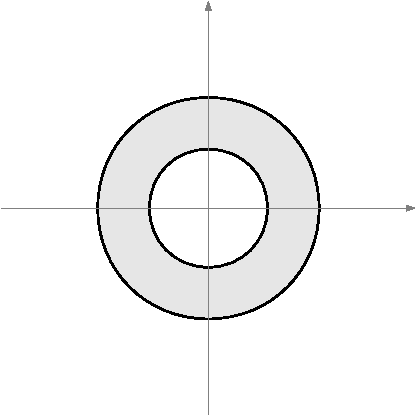
\includegraphics[width=0.45\textwidth]{curvelet_frequency_windows_radial_cropped}%
        \label{fig:curvelet_frequency_windows_radial}%
    }
    \quad
    \subfloat[Angular window]{%
        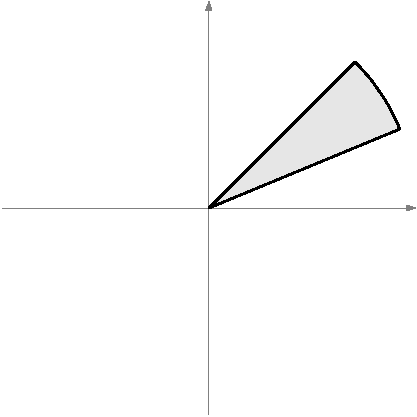
\includegraphics[width=0.45\textwidth]{curvelet_frequency_windows_angular_cropped}%
        \label{fig:curvelet_frequency_windows_angular}%
    }
    \quad
    \subfloat[Combined window]{%
        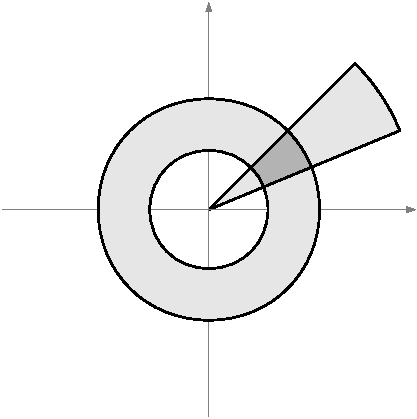
\includegraphics[width=0.45\textwidth]{curvelet_frequency_windows_combined_cropped}%
        \label{fig:curvelet_frequency_windows_combined}%
    }
    \quad
    \subfloat[Complete coronisation]{%
        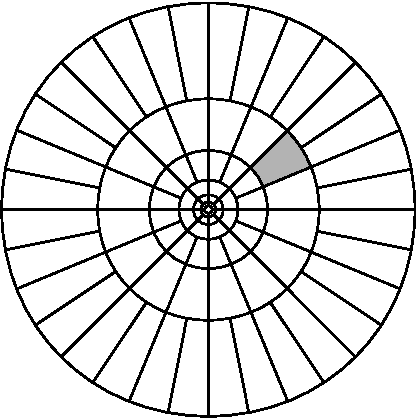
\includegraphics[width=0.45\textwidth]{curvelet_frequency_windows_corona_cropped}%
        \label{fig:curvelet_frequency_windows_corona}%
    }
    \caption[Curvelet frequency windows]{
        The window $W(2^{-j}r)$ at scale $2^j$
        \subref{fig:curvelet_frequency_windows_radial} is combined with the
        window $V(t)$ \subref{fig:curvelet_frequency_windows_angular} to form a
        support wedge for the curvelet
        \subref{fig:curvelet_frequency_windows_combined}. The wedge roughly
        obeys a $width \propto length^2$ relation.
        \subref{fig:curvelet_frequency_windows_corona} shows the wedge within a
        schema of the complete tiling in frequency domain.
    }
    \label{fig:curvelet_frequency_windows}
\end{figure}

The waveform $\varphi_j$ can then be expressed as being the inverse Fourier
transform of $\hat{\varphi}_j = U_j$ and all curvelets of a scale $2^{-j}$ can
be derived by
\begin{itemize}
    \item rotating $\varphi_j$ by a sequence of equispaced rotation angles
        $\theta_l = 2 \pi \cdot 2^{-\lfloor\frac{j}{2}\rfloor} \cdot l$ with $l
        = 0,1,\dots$ such that $0 < \theta_l < 2 \pi$ and
    \item translating $\varphi_j$ by a sequence of offsets $k = (k_1, k_2) \in \mathbb{Z}^2$:
\end{itemize}
\begin{equation} \label{eq:continuous_curvelet}
    \varphi_{j,k,l}(x) = \varphi_j(R_{\theta_l}(x - x_k^{(j,l)})),
\end{equation}
where $x = (x_1, x_2)$, $R_{\theta}$ is the rotation matrix for angle $\theta$
and $x_k^{(j,l)} = R_{\theta_l}^{-1}(k_1 \cdot 2^{-j}, k_2 \cdot
2^{-\frac{j}{2}})$.

\begin{figure}[h]
    \centering
    \subfloat[Coarse Curvelet waveform in time and frequency domain]{%
        \plotgraphics{curvelet_examples/curvelet_1_time.png}{194}{320}{194}{320}{$x_1$}{$x_2$}%
        \plotgraphics{curvelet_examples/curvelet_1_frequency.png}{0}{512}{0}{512}{$\omega_1$}{$\omega_2$}%
        \label{fig:curvelet_example_1}
    }
    \quad
    \subfloat[Fine Curvelet waveform in time and frequency domain]{%
        \plotgraphics{curvelet_examples/curvelet_2_time.png}{194}{320}{194}{320}{$x_1$}{$x_2$}%
        \plotgraphics{curvelet_examples/curvelet_2_frequency.png}{0}{512}{0}{512}{$\omega_1$}{$\omega_2$}%
        \label{fig:curvelet_example_2}
    }
    \caption[Curvelet waveforms in time and frequency domain]{
        Curvelet waveforms on coarse \subref{fig:curvelet_example_1} or fine
        \subref{fig:curvelet_example_2} scale with time domain shown on the
        left and frequency domain shown on the right side.
    }
    \label{fig:curvelet_examples}
\end{figure}


Each curvelet coefficient $c(j, l, k)$ can then be calculated as the inner
product of $f \in L^2(\mathbb{R}^2)$ and curvelet $\varphi_{j, l, k}$:
\begin{equation} \label{eq:continuous_curvelet_coefficient}
    c(j, l, k) := \langle f, \varphi_{j, l, k} \rangle = \int_{\mathbb{R}^2} f(x) \overline{\varphi_{j, l, k}(x)} dx
\end{equation}

As visible in figure \ref{fig:curvelet_frequency_windows_corona} curvelets also
have non-directional components at the coarsest scale, similar to those found
in the wavelet transform. Those curvelets will be defined using a special
low-pass filter window $W_0$, which is characterized as being the remainder of
the tiling not covered by the previously described radial windows:
\begin{equation*}
    |W_0(r)^2| + \sum_{j \geq 0} |W(2^{-j}r)|^2 = 1
\end{equation*}
With the help of window, defining the coarse scale curvelet $\varphi_{j_0, k}$
via its Fourier transform is straightforward:
\begin{equation} \label{eq:continuous_coarse_curvelet}
    \varphi_{j_0, k}(x) = \varphi_{j_0}(x-2^{-j_0}k), \hat{\varphi}_{j_0}(\omega) = 2^{-j_0}W_0(2^{-j_0}|\omega|),
\end{equation}
where $k = (k_1, k_2) \in \mathbb{Z}^2$.

Note that, in contrast to the Gabor wavelets (Figure \ref{fig:gabor_tiling}),
there is no gap in the curvelet tiling, so no information is lost.

\subsection{The Fast Discrete Curvelet Transform}\label{sec:background_fdct}

Based on the above definition of the continuous curvelet transform, a team
around the authors of the original curvelet publication presented two digital,
discrete implementations of the transform: the Fast Discrete Curvelet Transform
(FDCT) \autocite{candes_fast_2006}. The implementations have been described in
2D and 3D, but since this paper deals exclusively with 2D images, the
explanation below will also be restricted to two dimensions.

The digital versions of the transforms operate on arrays $f[t_1, t_2]$ with $0
\leq t_1, t_2 < n$ to produce coefficients $c^D(j, l, k)$ in a way
consistent with the continuous version (Equation
\ref{eq:continuous_curvelet_coefficient}):
\begin{equation}
    c^D(j, l, k) := \sum_{0 \leq t_1, t_2 < n} f[t_1, t_2] \overline{\varphi_{j, l, k}^D[t_1, t_2]}.
\end{equation}

Since the windows used in the continuous form are based on rotations and dyadic
coronae, they are not well suited for use with cartesian arrays. The discrete
formulation substitutes them with appropriate concepts. Instead of concentric
annuli, the window function $W^D_j$ generates concentric, square "rings" using
the square windows $\Phi_j(\omega_1, \omega_2) = \phi(2^{-j}\omega_1)
\phi(2^{-j}\omega_2)$, with $\phi$ being a low-pass 1D window:
\begin{equation*}
    W_j^D(\omega) = \sqrt{\Phi_{j+1}^2(\omega) - \Phi_j^2(\omega)}, \quad j \geq 0.
\end{equation*}
The rotation matrix $R_{\theta}$ is replaced by the shear matrix $S_{\theta}$
to create the combined window function
\begin{equation*}
    U_{j, l}^D := W_j^D(\omega) V_j(S_{\theta_l}\omega).
\end{equation*}
The sequence $\theta_l$ is defined as a sequence of equispaced slopes
$\tan(\theta_l) := l \cdot 2^{- \lfloor \frac{j}{2} \rfloor}$ with
$l=-2^{\lfloor \frac{j}{2} \rfloor}, \dots, 2^{\lfloor \frac{j}{2} \rfloor} -
1$.

Special attention must be paid to creating the windows, that touch the
diagonals, to ensure
\begin{equation*}
    \sum_{j} \sum_{l} | U_{j, l}^D (\omega)|^2 = 1
\end{equation*}
holds, so the tiling obeys the admissibility condition just like in the
continuous case. Figure \ref{fig:curvelet_frequency_windows_discrete} shows a
tiling of all $U_{j, l}^D$.

\begin{figure}[h]
    \centering
        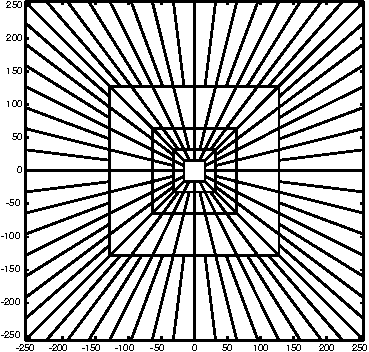
\includegraphics[width=0.5\textwidth]{curvelet_frequency_windows_discrete_cropped}
    \caption[Discrete frequency tiling using concentric squares]{
        Discrete frequency tiling using concentric squares (from Candes et al.\
        \autocite{candes_fast_2006})
    }
    \label{fig:curvelet_frequency_windows_discrete}
\end{figure}

\subsubsection{FDCT using unequispaced FFTs}

The first implementation of the discrete curvelet transform transfers the input
array $f[t_1, t_2]$, $0 \leq t_1, t_2 < n$ into the Fourier domain to obtain
$\hat{f}[n_1, n_2]$:
\begin{equation*}
    \hat{f}[n_1, n_2] = \sum_{t_1, t_2 = 0}^{n - 1} f[t_1, t_2] e^{- \frac{i 2 \pi (n_1 t_1 + n_2 t_2)}{n}}, \quad -\frac{n}{2} \leq n_1, n_2 < \frac{n}{2}
\end{equation*}

The obtained Fourier samples need to be interpolated for each pair of scale $j$
and angle $l$ to match the grid of the sheared support window $U_j^D[n_1, n_2]$
. The authors achieve this by resampling $\hat{f}$ on the grid
implied by the sheared window for each angle via a series of 1D fast Fourier
transforms.  These transforms represent a polynomial interpolation of each
"column" of the parallelogram $P_j$ containing the sheared window (Figure
\ref{fig:curvelet_usfft_tiling}), that can be computed with a $O(n^2 \log n)$
complexity in a sufficiently exact approximation.

This yields an object $\hat{f}[n_1, n_2 - n_1 \tan \theta_l]$ for $(n_1, n_2)
\in P_j$, that can be multiplied with the window $U_j^D$ described above in
order to create a localized "wedge" with the orientation $\theta_l$:
\begin{equation*}
    f_{j, l}^D[n_1, n_2] = \hat{f}[n_1, n_2 - n_1 \tan \theta_l] U_j^D[n_1, n_2]
\end{equation*}

The discrete curvelet coefficients $c^D(j, l, k)$ can then be calculated by
applying the inverse 2d Fourier transform:
\begin{equation*}
    c^D(j, k, l) = \sum_{n_1, n_2 \in P_j} \hat{f}[n_1, n_2 - n_1 \tan \theta_l] U_j^D[n_1, n_2] e^{i 2 \pi (\frac{k_1 n_1}{L_{1, j}} + \frac{k_2 n_2}{L_{2,j}})},
\end{equation*}
in which $L_{1, j}$ and $L_{2, j}$ are the length and width of the rectangle supporting $U_j^D$.

\begin{figure}[h]
    \centering
    \subfloat[Sheared USFFT tiling]{%
        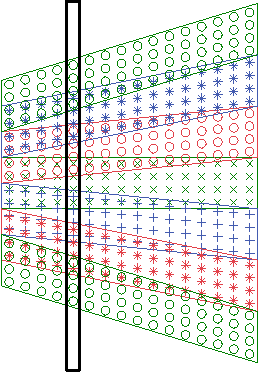
\includegraphics[width=0.35\textwidth]{curvelet_usfft_tiling_column_cropped}%
        \label{fig:curvelet_usfft_tiling}%
    }
    \quad
    \subfloat[Sheared tiling for wrapping]{%
        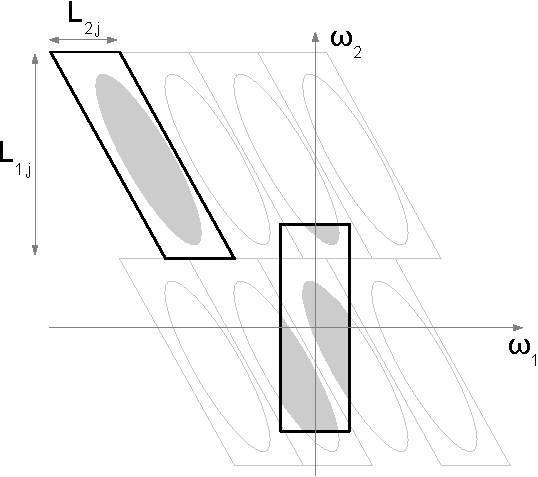
\includegraphics[width=0.55\textwidth]{curvelet_wrapping_cropped}%
        \label{fig:curvelet_wrapping_tiling}%
    }
    \caption[Frequency tilings for USFFT and wrapping]{
        \subref{fig:curvelet_usfft_tiling} illustrates the respective grid for
        each parallelogram containing the sheared support windows of the "east
        quadrant". The box highlights one of the columns, that represent one of
        the 1D polynomial interpolation problems solved for resampling.
        In \subref{fig:curvelet_wrapping_tiling} the parallelogram $P_{j ,l}$
        is shown on top of the tilted tiling of a curvelet in frequency domain.
        Due to the periodicity, the rectangle in the center contains the same
        curvelet, but has a much smaller axis aligned bounding box for the FFT
        to operate on. Both images have been adapted from Candes et al.\ 
        \autocite{candes_fast_2006}.
    }
    \label{fig:curvelet_discrete_tilings}
\end{figure}

\subsubsection{FDCT using wrapping}

As before, FDCT using wrapping first calculates $\hat{f}[n_1, n_2]$ with
$-\frac{n}{2} \leq n_1, n_2 < \frac{n}{2}$ as the Fourier transform of the
input $f$. The sample is then localized by multiplying it with a window $U_{j,
l}^D$ for each angle $j$ and scale $l$:
\begin{equation*}
    d_{j, l}[n_1, n_2] = U_{j, l}^D \hat{f}[n_1, n_2]
\end{equation*}

To avoid the computationally costly interpolation step required in the USFFT
approach, this method keeps the rectangular grid of the input signal. Because
an axis-aligned bounding box of the window $U_j^D$ in Fourier domain cannot
maintain the $width \propto length^2$ proportions of the window, applying an
inverse Fourier transform on such a bounding box in general would lead to
significant oversampling of the coefficients and thereby increase the memory
requirements for fine scale curvelets beyond that of the the USFFT approach. In
order to circumvent that, the authors utilize the periodic nature of the
Fourier transform and propose generating a periodically wrapped version of the
fourier samples. For $P_{j, l}$ as the bounding parallelogram of $U_{j, l}^D$,
$L_{1, j}$ and $L_{2, j}$ are the period lengths by which to translate $P_{j,
l}$ in the horizontal and vertical direction to produce a suitable tiling for
each orientation $\theta_l$ (Figure \ref{fig:curvelet_discrete_tilings}). Thus,
the wrapped, localized data are
\begin{equation*}
    f_{j, l}^D[n_1, n_2] = W d_{j, l}[n_1, n_2] = \sum_{m_1 \in \mathbb{Z}} \sum_{m_2 \in \mathbb{Z}} d_{j, l}[n_1 + m_1 L_{1, j}, n_2 + m_2 L_{2, j}]
\end{equation*}
with $0 \leq n_1 < L_{1, j}$ and $0 \leq n_2 < L_{2, j}$, which gives a
rectangle of size $L_{1, j}$ times $L_{2, j}$.

Again, the discrete curvelet coefficients $c^D(j, l, k)$ can then be collected
using the inverse 2d Fourier transform:
\begin{equation*}
    c^D(j, k, l) = \sum_{n_1, n_2 \in P_j} f_{j, l}^D[n_1, n_2] e^{i 2 \pi (\frac{k_1 n_1}{L_{1, j}} + \frac{k_2 n_2}{L_{2,j}})}.
\end{equation*}

\subsection{gPb Contour Detection}\label{sec:background_gpb}

Maire et al.\ \autocite{maire_using_2008} describe an improvement of the
contour detector published by Martin et al.\ \autocite{martin_learning_2004}
that includes global information in addition to local cues. The
orientation-specific local parameters $G_i$ extracted from a circular
neighborhood around the location $(x, y)$ are brightness, color and texture
gradients on three scales. They are summarized as a coefficient $mPb(x, y,
\theta)$ using a weighted sum with weights $\alpha_i$:
\begin{equation*}
    mPb(x, y, \theta) = \sum_{i=1}^9 \alpha_i G_i(x, y, \theta)
\end{equation*}

The global combonent $sPb(x, y, \theta)$ is the result of applying a
filterbank of directional gaussian derivatives to a set of $k$ generalized
eigenvectors $v_j$, $j \in 1, \dots, k$. The linear system these eigenvectors are
obtained from has an affinity matrix derived from the intervening contour cue
\autocite{fowlkes_learning_2003}. The linear combination of the individual
directional derivatives then represents the large-scale contours in the image:
\begin{equation*}
    sPb(x, y, \theta) = \sum_{j=1}^k \frac{1}{\sqrt{\lambda_j}} sPb_{v_j}(x, y, \theta)
\end{equation*}

A further linear combination of the local component $mPb$ and the global
component $sPb$ with learned weights $\alpha_i$ and $\gamma$ provides a
detailed map of contours in the image while limiting the amount of clutter
compared to a purely local contour detector:
\begin{equation*}
    gPb(x, y, \theta) = \sum_{i=1}^9 \alpha_i G_i(x, y, \theta) + \gamma \cdot sPb(x, y, \theta)
\end{equation*}

From these directional contour maps, Arbeláez et al.\ derived a hierarchical
contour detector \autocite{arbelaez_contours_2009}, that conditionally joins
adjacent regions to obtain closed-contour maps of high quality.
